\documentclass[]{article}
\usepackage{amssymb}
\usepackage[backend=bibtex,style=authoryear,natbib=true]{biblatex} % Use the bibtex backend with the authoryear citation style (which resembles APA)

\addbibresource{example.bib} % The filename of the bibliography

\usepackage[autostyle=true]{csquotes} % Required to generate language-dependent quotes in the bibliography

\usepackage{tikz}
\usepackage{tikz-network}
\usepackage{breqn}

\usepackage{graphicx}
\usepackage{subcaption}
\usepackage{multirow}
\usetikzlibrary{fit}
\usetikzlibrary {arrows.meta,graphs,shapes.misc}
\usetikzlibrary {positioning}

\newcommand{\bn}{\textbf{n}}
\newcommand{\tabhead}[1]{\textbf{#1}}

\begin{document}



\section{Guided Gated Convolution Neural Network for Normal Inference }

From the Figure \ref{fig:normal-histo-diff} we can observe the normal difference between ground-truth and GCNN predicted normals in another dimension. It separates the interval \left[ -1,1 \right], which is exactly the range of normal vector, to 256 sections. Then it counts the number of points locates in each section for 3 axes.  The 3 axes are fitted quit well in most of interval but other than \left[ -0.25,0.25 \right] for x and y axes and  interval close to $ -1 $ for z axis. Therefore a further constraint can be considered to the loss function related to the normal difference shown in this figure.

It is faulty that almost no normal has -1 z-component in GCNN predicted normal map. The reason?
\begin{figure}[h!]
	\centering
	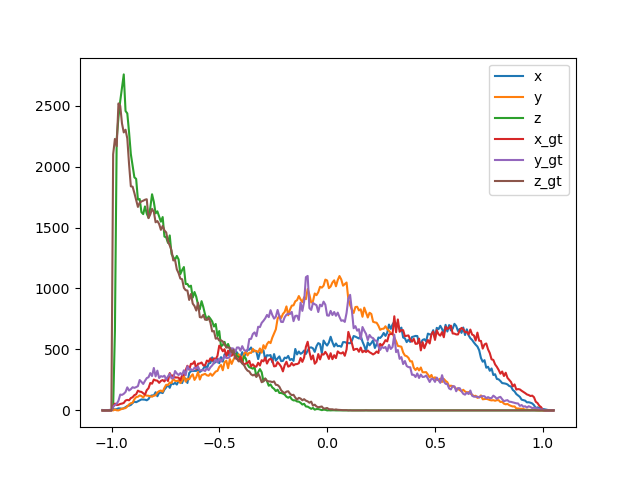
\includegraphics[width=\linewidth]{./Figures/normal-histo-diff/normal-histo-diff.png}
	\caption{The normal difference of between GCNN and ground-truth in x, y, z-axis respectively. The y axis indicates the number of points, x axis indicates the value of normal in x/y/z axis. (The chart is based on the "dragon" scene showing above)}
	\label{fig:normal-histo-diff}
\end{figure}


\end{document}
